\documentclass[
BCOR=5mm,           % Binderkorrektur von 5mm vorsehen
fontsize=11pt,      % Schriftgr��e 11 Punkte
oneside,            % Einseitig
parskip,            % Paragraphen nicht einrücken
headsepline,        % Kopfzeile nach unten durch Linie abgrenzen (scrheadings)
%footbotline,       % Fu�zeile nach unten durch Linie abgrenzen (scrheadings)
plainheadsepline,   % Kopfzeile nach unten durch Linie abgrenzen (scrplain)
plainfootbotline,   % Fu�zeile nach unten durch Linie abgrenzen (scrplain)
%headtopline,       % Kopfzeile nach oben durch Linie abgrenzen (scrheadings)
footsepline,        % Fu�zeile nach oben durch Linie abgrenzen (scrheadings)
plainheadtopline,   % Kopfzeile nach oben durch Linie abgrenzen (scrplain)
plainfootsepline,   % Fu�zeile nach oben durch Linie abgrenzen (scrplain)
]{scrbook}          % Koma-Script Klasse zum setzen eines Buchs


\usepackage{lmodern}

% Die "Standard-Header" f�r deutsche Dokumente
\usepackage[latin1]{inputenc}    % ISO-8859-1 bzw. Latin1 als Encoding
%\usepackage[T1]{fontenc}         % T1 Schriften verwenden (sieht besser aus)
\usepackage[ngerman]{babel}      % Neue deutsche Rechtschreibung 

% "Sch�nere" Schriften einbinden
%\usepackage{mathpazo}            % Serifen-Font mit passendem Math-Font
%\usepackage[scaled=.95]{helvet}  % Serifenloser Font passend zu mathpazo
%\usepackage{courier}             % "Sch�nerer" Festbreiten-Font

% Koma-Script Paket zum setzen vom Kopf- und Fu�zeilen einbinden
%\usepackage{scrpage2}
\usepackage{scrlayer-scrpage}
\RequirePackage{scrlfile}
\ReplacePackage{scrpage2}{scrlayer-scrpage}
\usepackage{substr}

%\pagestyle{scrheadings}
\clearpairofpagestyles
\automark[section]{chapter}

\ohead[\sffamily\scshape\bfseries\large\headmark]
{\sffamily\scshape\bfseries\large\headmark}

\ofoot[\sffamily\thepage]{\sffamily\thepage}

\usepackage{listings}
\lstset{
captionpos=b,                % Beschriftung unterhalb (bottom)
numbers=left,                % Zeilennummern links
frame=trbl,                  % Rahmen zeichnen (top, right, bottom, left)
basicstyle=\small\ttfamily,  % Festbreitenschrift verwenden (small)
language=Java                % Sprache auf Java einstellen
}

\usepackage[ngerman]{translator}

\usepackage[
nonumberlist, % Keine Seitenzahlen anzeigen
acronym,      % Abkürzungsverzeichnis erstellen
toc,          % In Inhaltsverzeichnis aufnehmen
%section       % Verzeichniseintrag als Section
]{glossaries}

% Ein eigenes Verzeichnis definieren (Smbolverzeichnis)
% Das Stichwort- und Abkürzungsverzeichnis wird analog vordefiniert
% Siehe makeindex Aufrufe - Hier werden die Dateiendungen festgelegt
\newglossary[slg]{symbolslist}{syi}{syg}{Symbolverzeichnis}

\makeglossaries


% Paket zum generieren von Blindtext
\usepackage{blindtext}

% Paket zum Einbinden von Bildern
\usepackage{graphicx}

%              
% WORKAROUND, damit lstlistoflistings funktioniert:
% Quelle: http://www.komascript.de/node/477
%
\makeatletter
\@ifundefined{float@listhead}{}{%
    \renewcommand*{\lstlistoflistings}{%
        \begingroup
    	    \if@twocolumn
                \@restonecoltrue\onecolumn
            \else
                \@restonecolfalse
            \fi
            \float@listhead{\lstlistlistingname}%
            \setlength{\parskip}{\z@}%
            \setlength{\parindent}{\z@}%
            \setlength{\parfillskip}{\z@ \@plus 1fil}%
            \@starttoc{lol}%
            \if@restonecol\twocolumn\fi
        \endgroup
    }%
}
\makeatother

% ------------------------------------------------------------------------
% LaTeX - Preambel ******************************************************
% ------------------------------------------------------------------------
% pre-work
% ========================================================================
% % ToDo kennzeichnen
\newcommand{\workTodo}[1]{\textcolor{red}{todo: #1}}

% % Für Datum und Zeit in Fusszeile
% % !!!Inhalt bei Fertigstellung der Arbeit löschen
\newcommand{\workMarkDateTime}{\today{}}

% % Alle Namen werden im Titel und im hyperref-Paket eingetragen
% % !!! Ueberall für <Wert> das Entsprechende eintragen

% <Fakultaet> In Welcher Fakultät wurde die Arbeit erstellt 
\newcommand{\workFakultaet}{Informatik und Informationstechnik}

% <Typ> Studienarbeit, Dipolmarbeit, Studienarbeit oder Bachlor-Abschlussarbeit
\newcommand{\workTyp}{Studienarbeit}

% <Studiengang> z.B. Kommunikationstechnik
\newcommand{\workStudiengang}{Technische Informatik}

% <Titel> der Arbeit
\newcommand{\workTitel}{Visualisierung eines echtzeitf\"ahigen Routenplan-Algorithmus}

% <Semester> mit Jahr z.B. Sommersemester 2008  
\newcommand{\workSemester}{Sommersemester 2023}

% <Name> des Studenten
\newcommand{\workNameStudent}{Seid Jadadic}

% <Pruefer> Name des prüfenden (betreuenden) Professor an der Hochschule
\newcommand{\workErstPruefer}{Prof. Dr. Reiner Marchthaler} 

% <Zweitprüfer>
\newcommand{\workZweitPruefer}{Prof. Dr. J\"urgen Koch}

% %%% Nur bei Abschluss-Arbeiten

% <Datum> der Abgabe der Arbeit (Eidesstatliche Erklärung)
\newcommand{\workDatum}{\today\xspace}

% <Ort> Standort der erstellten Arbeit 

\newcommand{\workOrt}{Esslingen}

% <Zeitraum>
\newcommand{\workZeitraum}{\workTodo{<Zeitraum>}\xspace}


% %%% Nur bei Industrie-Arbeiten:

% <Firma>
\newcommand{\workFirma}{\workTodo{<Firma>}\xspace}

% <Betreuer in der Firma>
\newcommand{\workFirmenBetreuer}{\workTodo{<Betreuer in der Firma>}\xspace}

% Firmenlogo Name hier anpassen, Größe (wenn möglich) nicht ändern
\newcommand{\workFirmenLogo}{\includegraphics[width=5cm]{fig/aa-titel/Bosch_4C_S}} 


%Abk�rzungen
%\newacronym{acr:POJO}{POJO}{Plain Old Java Object}
%\glsadd{acr:POJO}

% Beginn des eigentlichen Dokuments

\begin{document}

% Titelseite (verwendet pagestyle=empty)
\begin{titlepage}
\begin{center}

\includegraphics[scale=0.6]{bilder/he_logo.jpg}\\
\vspace{0.5cm} Fakult�t \workFakultaet\\
\vspace{0.5cm} Studiengang \workStudiengang\\
\vspace{1.5cm} \workTyp\\
\vspace{0.5cm} \Large Bachelor of Engineering\\
\vspace{1.5cm} \Huge \workTitel\\
\vspace{1.5cm} \Large \workNameStudent\\\normalsize
\vspace{0.5cm} \workSemester\\\normalsize
\vfill{}
\begin{tabular}{rl}
%Firma: & Gro�e Firma GmbH\\[0.5cm]
%Betreuer: & Dipl. Ing. (FH) Max Betreuer\\[0.5cm]
% Erstpr�fer: & Prof. Dr. Hans Wissenschaftler\\
Erstpr�fer: & \workErstPruefer \\
Zweitpr�fer: & \workZweitPruefer\\
\end{tabular}
\end{center}
\end{titlepage}

% Erkl�rung
\chapter*{Erkl�rung}
\thispagestyle{empty}
Hiermit erkl�re ich, dass ich die vorliegende Arbeit selbstst�ndig angefertigt habe. Es wurden nur die in der Arbeit ausdr�cklich benannten Quellen und Hilfsmittel benutzt. W�rtlich oder sinngem�� �bernommenes Gedankengut habe ich als solches kenntlich gemacht.
\vspace{1cm}
\begin{center}
	\begin{tabular}{lp{2cm}p{5.5cm}}
		& & \multirow{2}{*}{
\includegraphics[width=5cm]{bilder/unterschrift.jpg}} \\
		\workOrt, \workMarkDateTime & & \\
		\cline{1-1}\cline{3-3}
		Ort, Datum &  & \workNameStudent\\
	\end{tabular}
\end{center}

% "Frontmatter" beginnen (Formatierung umschalten)
% Platz f�r Inhaltsverzeichnis und anderes
\frontmatter

% Inhaltsverzeichnis ausgeben (aktualisierung erst beim zweiten Mal!)
\tableofcontents

% Definiert die deutschen Eintr�ge im Inhaltsverzeichnis
% Direkt vor \printglossary einbinden
\deftranslation[to=German]{Acronyms}{Abk�rzungsverzeichnis}
\deftranslation[to=German]{Glossary}{Stichwortverzeichnis}

% Die �berschrift f�r den Eintrag mit title= �berschreiben
% Ohne Angabe des type wird type "glossary" verwendet
% Ausser "altlist" existieren einige andere Stile wie z.B. "long"
\printglossary[style=altlist, title=Stichwortverzeichnis]
\newpage

% Das Abk�rzungsverzeichnis hat den Typ \acronymtype
%\printglossary[type=\acronymtype, style=long, title=Abk�rzungsverzeichnis]
%\newpage

% Das selbstdefinierte Verzeichnis ausgeben
%\printglossary[type=symbolslist, style=long, title=Symbolverzeichnis]
%\newpage  

% Hauptteil beginnen (Formatierung umschalten)
\mainmatter

%------------------------------------------------------------------
%                      Kapitelstruktur einf�gen
%------------------------------------------------------------------

\chapter{Einleitung}

In diesem Kapitel wird die Motivation f�r die Wahl dieses Themas erl�utert und die Zielsetzung der Studienarbeit festgelegt. Zudem wird ein �berblick �ber den Aufbau und den Inhalt der Arbeit gegeben.
\section{Motivation}
Die vorliegende Studienarbeit befasst sich mit der Implementierung und Evaluierung des A*-Routenplanungsalgorithmus, einem leistungsf�higen und vielseitig einsetzbaren Routenplanungsalgorithmus. \\
F�r die Wahl dieses Themas gibt es mehrere Gr�nde, die im Folgenden erl�utert werden.

Effiziente Routenplanung spielt in vielen Anwendungsbereichen eine entscheidende Rolle. Von Navigationssystemen und Logistik bis hin zu Robotik und Videospielen sind viele Systeme auf eine schnelle und zuverl�ssige Wegfindung angewiesen. \\
Der A*-Algorithmus hat sich dabei als eines der besten Verfahren erwiesen und wird daher in der Praxis h�ufig eingesetzt.

Die Motivation hinter der Implementierung des A*-Algorithmus ist es, ein grundlegendes Verst�ndnis f�r diesen Algorithmus zu entwickeln und die zugrundeliegenden Konzepte zu erforschen. Die Arbeit soll es erm�glichen, die Funktionsweise des A*-Algorithmus praktisch in C++ umzusetzen und dadruch einen tieferen Einblick in die Arbeitsweise von Routing-Algorithmen zu gewinnen. 
\newpage
Ein weiterer Aspekt dieser Arbeit liegt in der M�glichkeit, die Leistungsf�higkeit des A*-Algorithmus unter verschiedenen Bedingungen zu evaluieren. Dabei sollen sowohl einfache auch komplexe Graphen analysiert werden, um den Einfluss von Graphengr��e und -struktur auf die Laufzeit des Algorithmus zu untersuchen. Der Vergleich mit anderen Routingalgorithmen erlaubt es au�erdem, die Vor- und Nachteile des A*-Algorithmus gegen�ber alternativen Ans�tzen zu diskutieren. 

\section{Zielsetzung der Studienarbeit}
Das Hauptziel dieser Arbeit ist es, den A*-Algorithmus in C++ zu implementieren und seine Funktionsweise zu verstehen. Dabei werden die verschiedenen Komponenten des Algorithmus untersucht, wie z.B. die Heuristik, sowie die Datenstrukturen.

Ein weiterer Aspekt ist die Bewertung der Leistungsf�higkeit des A*-Algorithmus. \\
Es werden verschiedene Tests durchgef�hrt, um die Laufzeit des Algorithmus auf verschiedenen Graphen zu messen und zu vergleichen.

Die Erkenntnisse aus dieser Studienarbeit sollen dazu dienen, die Funktionsweise des A*-Algorithmus besser zu verstehen und seine Leistungsf�higkeit in verschiedenen Anwendungsf�llen zu bewerten. Die Ergebnisse k�nnen wertvolle Informationen liefern, um den A*-Algorithmus in verschiedenen Bereichen effektiv einzusetzen und m�gliche Optimierungsm�glichkeiten aufzuzeigen.

\section{Aufbau der Studienarbeit}
Die vorliegende Studienarbeit befasst sich mit der Implementierung eines A*-Routenplan Algorithmus und untersucht dessen Leistungsf�higkeit in verschiedenen Szenarien. 

In der Einleitung wird die Motivation f�r die Themenwahl erl�utert und die Zielsetzung der Studienarbeit definiert. Hier wird ein �berblick �ber die Problemstellung gegeben und die Vorgehensweise in der Arbeit beschrieben. 

\newpage
Im Abschnitt \glqq Grundlagen \grqq{} werden die grundlegenden Konzepte und Begriffe erl�utert, die f�r das Verst�ndnis des A*-Algorithmus und seiner Implementierung relevant sind. 

Der Abschnitt \glqq Datenstrukturen und Implementierungsdetails\grqq{} befasst sich mit den technischen Aspekten der Implementierung. Hier wird erl�utert, wie eine GraphML-Datei eingelesen wird und wie der A*-Algorithmus konkret implementiert wurde.\\ Es werden relevanten Datenstrukturen und Funktionen erl�utert, die f�r die Implementierung des Algorithmus ben�tigt werden. 

Die \glqq Evaluierung und Performance-Analyse\grqq{} bilden den vierten Abschnitt der Arbeit. Hier werden verschiedene Testf�lle vorgestellt, die das Einlesen der GraphML-Datei und die Implementierung des Algorithmus �berpr�fen. Au�erdem wird ein Vergleich der Laufzeiten des A*-Algorithmus auf verschiedenen Graphen durchgef�hrt, um die Performance in verschiedenen Szenarien zu bewerten. 

Im abschlie�enden Abschnitt werden die Ergebnisse und Erkenntnisse der Studienarbeit zusammengefasst. 

Der Anhang der Studienarbeit enth�lt die Quellcodes der implementierten Funktionen sowie die Unit-Tests zur �berpr�fung der Implementierung. 
\chapter{Grundlagen}
Die grundlegenden Konzepte und Techniken des A*-Algorithmus bilden das Fundament f�r das Verst�ndnis und die Implementierung eines effizienten Routenplanungsalgorithmus. In diesem Kapitel werden die wichtigsten Aspekte des A*-Algorithmus behandelt, darunter die Verwendung von Heuristiken und die Funktionsweise des \\
Algorithmus. 

\section{A*-Algorithmus}
Der A*-Algorithmus ist ein leistungsf�higer und weit verbreiteter Algorithmus f�r die Routenplanung in Graphen. Er kombiniert geschickt die Verwendung von Heuristiken mit einer Suche in der Breite oder in der Tiefe, um den besten Weg zwischen einem Startknoten und einem Zielpunkt zu finden. 

Entwickelt wurde der Algorithmus 1968 von Peter Hart, Nils Nilsson und Bertram Raphael. Der Name A* ist eine Anspielung auf die verwendete Bewertungsfunktion, die die Sch�tzung des k�rzesten Weges von einem gegebenen Knoten zu einem Zielknoten unter Ber�cksichtigung des bereits zur�ckgelegten Weges ber�cksichtigt. \cite{noauthor_-algorithmus_2022-1}

Der A*-Algorithmus kombiniert die Vorteile des Dijkstra-Algorithmus und des Best-First-Search-Algorithmus. Er arbeitet, indem er die Knoten des Graphen systematisch durchsucht und dabei den bisher geringsten Kosten von einem Startknoten zu jedem besuchten Knoten folgt. Dazu verwendet er eine Heuristik, die die verbleibenden Kosten vom aktuellen Knoten bis zum Zielknoten absch�tzt. Diese Heuristik ist die entscheidende Komponente, die es dem A*-Algorithmus erm�glicht, effizientere Such\-pfade zu finden, indem vielversprechende Pfade bevorzugt und weniger vielversprechende Pfade ignoriert werden.

W�hrend des Suchvorgangs berechnet der A*-Algorithmus f�r jeden Knoten $x$ 
\begin{equation}
	f(x) = g(x) + h(x)
\end{equation}
wobei $g(x)$ die bisherige Kostenfunktion vom Startknoten zum Knoten $x$ und $h(x)$ die Heuristik zur Sch�tzung der Kosten vom Knoten $x$ zum Zielknoten ist. Durch die Wahl des Knotens mit dem kleinsten $f(x)$ wird sichergestellt, dass der Algorithmus den k�rzesten Weg findet. \cite{russell_artificial_2010}
% Quelle vom Buch verwenden


Es ist jedoch zu beachten, dass die Effizienz und Genauigkeit des A*-Algorithmus stark von der verwendeten Heuristik abh�ngt. Eine gut gew�hlte Heuristik kann die Suche beschleunigen, w�hrend eine schlechte Heuristik m�glicherweise nicht die optimale L�sung liefert oder die Laufzeit des Algorithmus erh�ht.


\section{Heuristiken im A*-Algorithmus}
Ein zentraler Aspekt des A*-Algorithmus ist die Verwendung von Heuristiken, um den Suchraum effizienter zu durchsuchen. Eine Heuristik ist eine Funktion, die eine Sch�tzung des verbleibenden Aufwands f�r die Erreichung des Zielpunkts liefert. \\
Sie wird verwendet, um die Auswahl der n�chsten Knoten zu beeinflussen und somit den Algorithmus auf den vielversprechendsten Pfad zu bringen. \cite{russell_artificial_2010}
%Quelle vom Buch  

\subsection{Manhattan-Heuristik}
Die Manhattan-Heuristik verwendet die Summe der absoluten Differenzen der Koordinaten zweier Punkte. Sie misst die horizontale und vertikale Entfernung zwischen den Punkten und vernachl�ssigt dabei diagonale Bewegungen. Die Manhattan-Heuristik ist in Situationen n�tzlich, in denen nur horizontale und vertikale Bewegungen erlaubt sind, wie zum Beispiel in Schachbrettmustern.

\subsection{Euklidische-Heuristik}
Die Euklidische-Heuristik verwendet den euklidischen Abstand zwischen zwei Punkten in einem Kartesischen Koordinatensystem. Sie ist in Situationen n�tzlich, in denen es eine klare r�umliche Struktur gibt und Bewegungen in beliebigen Richtungen m�glich sind.

\subsection{Wahl einer Heuristik}
Die Wahl der Heuristik h�ngt von der spezifischen Anwendung ab und kann einen erheblichen Einfluss auf die Effizienz und Genauigkeit des A*-Algorithmus haben.
Um zu entscheiden, welche Heuristik besser geeignet ist, sollte man die spezifischen Anforderungen und Eigenschaften des Problems ber�cksichtigen.

\begin{figure}[h]
	\centering
	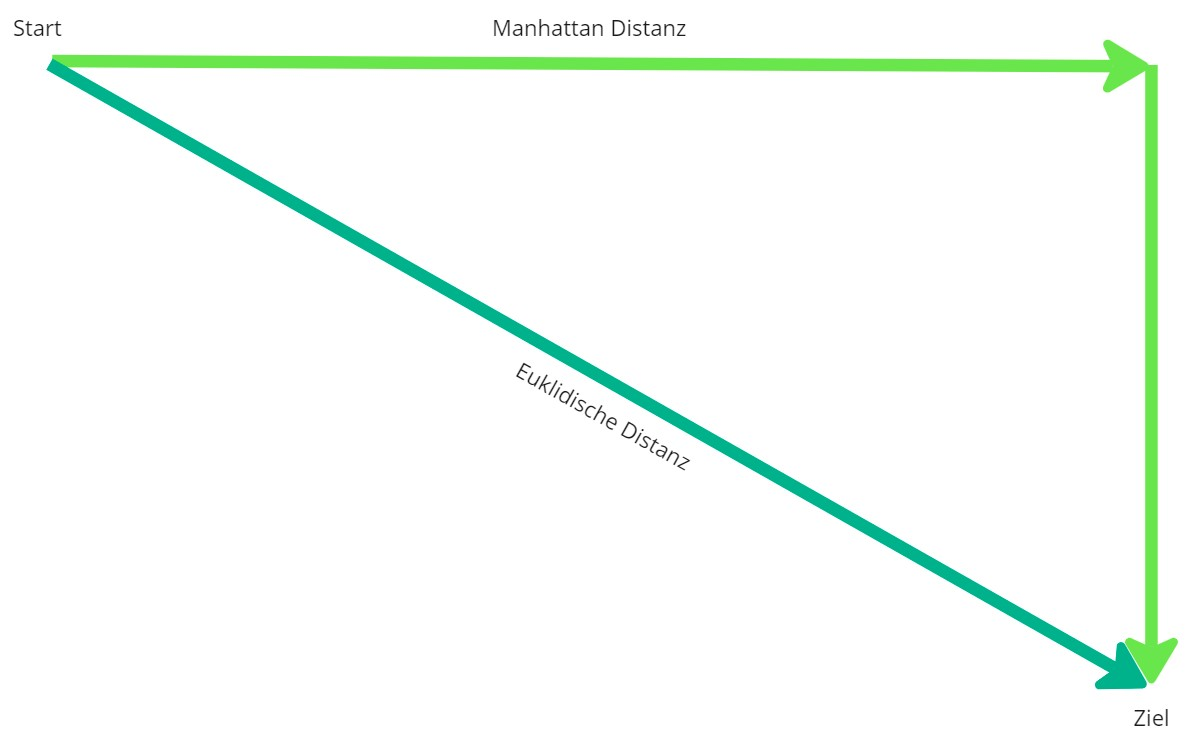
\includegraphics[scale=0.4]{bilder/Vergleich_Manhattan-Euklidisch.jpg}
	\caption{Vergleich der Heuristiken}
	\label{fig:vglManEuk}
\end{figure}

\newpage
In Abbildung \ref{fig:vglManEuk} kann man sehr gut den Unterschied der beiden Heuristiken erkennen. Wenn die Bewegung in beliebigen Richtungen stattfinden k�nnen und die r�umliche Struktur wichtig ist, liefert die euklidische-Heuristik eine bessere Sch�tzung. Wenn jedoch nur horizontale und vertikale Bewegungen m�glich sind oder die r�umliche Struktur diskret ist, ist die Manhattan-Heuristik angemessener. \\
Da ein Routenplanungsalgorithmus nicht auf horizontale und vertikale Bewegungen beschr�nkt sein sollte, ist die euklidische Heuristik f�r diesen Anwendungsfall die bessere Wahl.

\section{Vergleich mit anderen Routenplanalgorithmen}
Die Routenplanung ist ein grundlegendes Problem in vielen Anwendungsbereichen, und es gibt verschiedene Algorithen, die entwickelt wurden, um dieses Problem zu l�sen. In diesem Abschnitt wird der A*-Algorithmus mit anderen bekannten Routenplanungsalgorithmen verglichen und seine St�rken und Schw�chen aufgezeigt.

\subsection{Dijkstra-Algorithmus}
Der Dijkstra-Algorithmus ist einer der �ltesten und am h�ufigsten verwendeten Algorithmen f�r die Routenplanung in gewichteten Graphen. Er findet den k�rzesten Weg von einem Startknoten zu allen anderen Knoten im Graphen. Im Gegensatz zum A*-Algorithmus verwendet der Dijkstra-Algorithmus keine Heuristiken, sondern durchl�uft alle Knoten, um den k�rzesten Pfad zu finden \cite{sedgewick_algorithms_2011}. Dies f�hrt dazu, dass der Dijkstra-Algorithmus bei gro�en Graphen, insbesondere bei Graphen mit vielen Knoten, langsamer sein kann als der A*-Algorithmus.
%quelle von Buch Algorithms

\newpage
\subsection{Bellman-Ford-Algorithmus}
Der Bellman-Ford-Algorithmus ist ein weiterer bekannter Algorithmus, der ebenfalls mit gewichteten Graphen arbeitet. Im Gegensatz zum Dijkstra-Algorithmus kann der Bellman-Ford-Algorithmus jedoch auch mit Graphen umgehen, die negative Kantenl�ngen enthalten. Dies macht ihn zu einer geeigneten Wahl in bestimmten Situat\-ionen, in denen der A*-Algorithmus m�glicherweise nicht angewendet werden kann. \\
Allerdings ist der Bellman-Ford-Algorithmus in der Regel langsamer als der A*-Algori\-thmus, insbesondere bei gro�en Graphen.

\subsection{Greedy Best-First-Search}
Greedy Best-First-Search ist ein weiterer heuristischer Algorithmus, der f�r die Routenplanung verwendet werden kann. �hnlich wie der A*-Algorithmus verwendet er eine Heuristik, um die Auswahl der n�chsten Knoten zu beeinflussen. Allerdings verwendet Greedy Best-First-Search ausschlie�lich die Heuristik, ohne die bisherigen Kosten zu ber�cksichtigen. Dies f�hrt dazu, dass Greedy Best-First-Search m�glicherweise nicht den optimalen Pfad findet und zu suboptimalen Ergebnissen f�hren kann. \cite{noauthor_greedy_2022}
%quelle GeeksforGeeks

\subsection{Breitensuche (BFS) und Tiefensuche (DFS)}
Breitensuche und Tiefensuche sind einfache Suchalgorithmen, die auch f�r die Routenplanung verwendet werden k�nnen. Sie durchsuchen den Graphen schrittweise, ohne Heuristiken oder Kosten zu ber�cksichtigen. Obwohl diese Algorithmen einfach zu implementieren sind, sind sie m�glicherweise nicht die effizienteste Wahl f�r die Routenplanung in gro�en Graphen, da sie den Suchraum nicht effizient durchsuchen.

\chapter{Datenstrukturen und Implementierungsdetails}

\section{Einlesen einer GraphML-Datei}
Dieses Kapitel behandelt das Einlesen einer GraphML-Datei und die Strukturierung der darin enthaltenen Knoten- und Kanteninformation. \\
GraphML ist ein XML-basiertes Dateiformat, das h�ufig zur Darstellung von gerichteten und ungerichteten Graphen verwendet wird. Die Verarbeitung von GraphML-Dateien ist in verschiedenen Anwendungsbereichen wie Netzwerkvisualisierung, soziale Netzwerkanalyse oder Routenplanung unerl�sslich. 

Das Kapitel beginnt mit einer Analyse der GraphML-Struktur, um ein Verst�ndnis daf�r zu entwickeln, wie die Knoten- und Kanteninformationen in der Datei organisiert sind. Darauf aufbauend werden die Funktionen und Variablen in der Header-Datei \glqq car\_readFile.hpp\grqq{} erl�utert, die Teil der Klasse ReadFile sind. Diese Klasse wurde speziell entwickelt, um die GraphML-Datei zu �ffnen, zu lesen und die darin enthaltenen Daten effizient in einer unordered\_map zu speichern. 

Die Details der Implementierung der Klasse sind in der Datei \glqq car\_readFile.cpp\grqq{} beschrieben. Die Methode readFile() spielt eine zentrale Rolle und erm�glicht es, die Informationen aus der GraphML-Datei zu extrahieren und in der Datenstruktur abzulegen.  

\subsection{Struktur einer GraphML-Datei}
Die Struktur einer GraphML-Datei ist in Abbildung \ref{fig:graphmldat} dargestellt. Es handelt sich um ein XML-Dokument, das Informationen �ber einen gerichteten Graphen enth�lt. Jeder Knoten des Graphen wird durch eine eindeutige ID identifiziert. F�r jeden Knoten gibt es zwei Schl�ssel, die jeweils den x- und y-Koordinaten des Knotens entsprechen. \\
Der Wert des Schl�ssels \glqq d0\grqq{} gibt die x-Koordinate des Knotens an, w�hrend der Wert des Schl�ssels \glqq d1\grqq{} die y-Koordinate des Knotens angibt.

\begin{figure}[h]
	\centering
	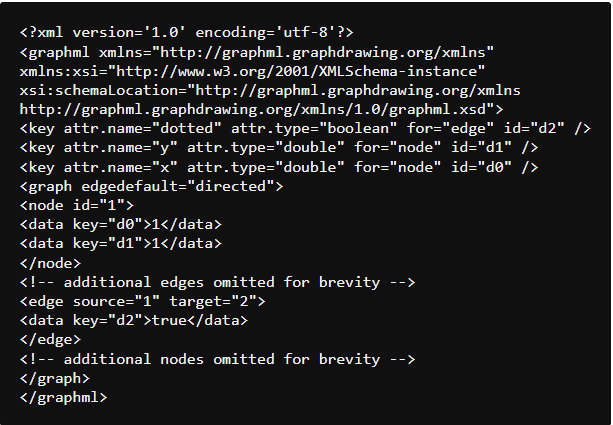
\includegraphics[scale=0.8]{bilder/graphml_datei.png}
	\caption{Struktur einer GraphML-Datei}
	\label{fig:graphmldat}
\end{figure}

Es gibt auch einen Kantenschl�ssel (\glqq d2\grqq{}), der einen booleschen Wert enth�lt, der angibt, ob die Fahrbahn mehrspurig ist oder nicht. Damit ist ein Spurwechsel m�glich. Der Graph selbst ist als \glqq gerichtet\grqq{} definiert, was bedeutet, dass jeder Knoten des Graphen Kanten zu anderen Knoten hat, diese Kanten aber nur in eine Richtung verlaufen.

\subsection{Die Header-Datei \glqq car\_readFile.hpp\grqq{} und ihre Funktionen}

Die Header-Datei enth�lt die Definitionen der Klasse ReadFile, die zum Lesen und Verarbeiten von GraphML-Dateien verwendet wird. Die Datei beginnt mit Pr�prozessor-\\anweisungen, um ein mehrfaches Einbinden der Datei zu verhindern. Anschlie�end werden verschiedene Header-Dateien der Standardbibliothek eingebunden, die f�r die Funktionalit�t der Klasse erforderlich sind. Die ReadFile-Klasse selbst ist in der Datei definiert.
\subsubsection{Datenstruktur \glqq NodeData\grqq}
Vor der Definition der Klasse ReadFile wird die Datenstruktur \glqq NodeData\grqq{} definiert, die Informationen �ber einen Knoten im Graphen enth�lt. Ein \glqq NodeData\grqq-Objekt besteht aus drei Attributen: 
\begin{itemize}
	\item \glqq m\_id\grqq{}: Eine 16-Bit unsigned Integer-Variable zur Speicherung der x- und y-Koordinaten des Knotens.  
	\item \glqq m\_x\grqq{} und \glqq m\_y\grqq{}: Float-Variablen zur Speicherung der x- und y-Koordinaten des Knotens. 
	\item \glqq connectedNodes\grqq{}: Ein Vektor von Integerwerten, der die IDs der Knoten enth�lt, die mit diesem Knoten verbunden sind. 
\end{itemize}

Die Struktur enth�lt auch einen Konstruktor, um die Initialisierung von \glqq NodeData\grqq-Objekten mit den gegebenen Werten zu erleichtern, sowie einen �berladenen Operator \glqq $<$\grqq{}, um die Sortierung der Knoten nach ihrer ID zu erm�glichen.
\newpage
\subsubsection{Klasse \glqq ReadFile\grqq}
Die Klasse selbst ist nun definiert. Sie enth�lt verschiedene �ffentliche und gesch�tzte Methoden und Variablen zum Lesen und Speichern von GraphML-Daten.\\
Es stehen zwei Konstruktoren zur Verf�gung: \\
Der Standardkonstruktor \glqq ReadFile()\grqq{} initialisiert die Variable \glqq m\_filename\grqq{} mit einem vorgegebenen Dateinamen \glqq c\_filename\grqq{}. \\
Der zweite Konstruktor \glqq ReadFile(string filename)\grqq{} akzeptiert einen Dateinamen als Parameter und weist diesen der Variablen \glqq m\_filename\grqq{} zu.

Die �ffentlichen Methoden sind: 
\begin{enumerate}
	\item \glqq readFile()\grqq{}: Dies ist der Hauptteil der Klasse, in dem die GraphML-Datei ge�ffnet, gelesen und die Knoten und Kanten in einer \glqq unordered\_map\grqq{} namens \glqq m\_nodes\grqq{} gespeichert werden.
	
	\item \glqq setFilename(string filename)\grqq{}: Mit dieser Methode kann der Dateiname der GraphML-Datei nachtr�glich ge�ndert werden.
	
	\item \glqq getNodes()\grqq{}: Diese Methode gibt eine \glqq unordered\_map\grqq{} zur�ck, das die Informationen �ber die gelesenen Knoten enth�lt.
\end{enumerate}

Die gesch�tzte Methoden dienen dazu, bestimmte Teile des Leseprozess f�r Knoten und Kanten aus der GraphML-Datei zu isolieren und zu verarbeiten.
\begin{enumerate}
	\item \glqq readNodeDataFromFile()\grqq{}: Diese Methode extrahiert die Daten eines einzelnen Knotens aus der GraphML-Datei. Sie liest die Zeilen der Datei, bis die Daten des Knotens vollst�ndig gelesen sind und speichert sie dann im Objekt \glqq m\_currentNode\grqq{} vom Typ \glqq NodeData\grqq{}.
	
	\item \glqq readEdgeDataFromFile()\grqq{}: Diese Methode extrahiert die Daten einer einzelnen Kante aus der GraphML-Datei. Sie liest die Zeilen der Datei, bis die Daten der Kante vollst�ndig gelesen sind und aktualisiert dann die Verbindungen des entsprechenden Quellknotens in der \glqq unordered\_map\grqq{}.
\end{enumerate}
\newpage
Die gesch�tzten Variablen werden verwendet, um tempor�re und w�hrend des Lesens relevante Daten zu speichern. 

\begin{enumerate}
	\item \glqq m\_currentNode\grqq{}: Ein Objekt vom Typ \glqq NodeData\grqq{}, das die Daten eines Knotens tempor�r speichert, w�hrend sie aus der Datei gelesen werden.
	
	\item \glqq m\_nodes\grqq{}: Eine \glqq unordered\_map\grqq{}, die die Informationen �ber die gelesenen Knoten speichert. Der Schl�ssel ist die ID des Knotens (uint16\_t) und der Wert ist das entsprechende \glqq NodeData\grqq{}-Objekt. 
	
	\item \glqq graphMlFile\grqq{}: Ein Dateistream, der die GraphML-Datei repr�sentiert, die zum Lesen der Daten ge�ffnet wird.
	
	\item \glqq m\_filename\grqq{}: Eine Zeichenkette, die den Dateinamen der GraphML-Datei enth�lt.
	
	\item \glqq m\_currentLine\grqq{}: Eine Zeichenkette, die die aktuelle Zeile darstellt, w�hrend die Datei Zeile f�r Zeile durchlaufen wird.
\end{enumerate}

\subsection{Implementierung des GraphML-Einleseprozess}
Die Methode \glqq ReadFile::readFile()\grqq{} bildet den Hauptteil der Implementierung und ist f�r das eigentliche Einlesen der GraphML-Datei verantwortlich. Sie �ffnet die GraphML-Datei mit dem in \glqq m\_filename\grqq{} gespeicherten Namen und geht diese Zeile f�r Zeile durch. Dabei werden die Informationen �ber jeden Knoten und jede Kante extrahiert und in \glqq m\_nodes\grqq{} gespeichert. Diese Datenstruktur erm�glicht einen schnellen Zugriff auf die Graphendaten und erleichtert sp�tere Analysen. 

Zun�chst wird die GraphML-Datei ge�ffnet, deren Name in der Member-Variablen \glqq m\_filename\grqq{} gespeichert ist. Dies erm�glicht den Zugriff auf die in der Datei enthaltenen Daten. Das �ffnen erfolgt �ber den C++-Standard-Dateistream fstream, der zum Lesen und Schreiben von Dateien verwendet wird. Dabei wird die Datei im Lesemodus (d.h. als Eingabedatei) ge�ffnet, um ihren Inhalt lesen zu k�nnen. Nach dem Aufruf von \glqq open()\grqq{} ist die GraphML-Datei ge�ffnet und der Datei-Stream \glqq graphMlFile\grqq{} kann auf die Datei zugreifen.
\newpage
Kann die Datei nicht erfolgreich ge�ffnet werden, z.B. weil sie nicht existiert oder die Zugriffsrechte fehlen, wird eine Fehlermeldung ausgegeben und eine Exception geworfen, um den ordnungsgem��en Ablauf zu gew�hrleisten. 

Anschlie�end wird die Datei Zeile f�r Zeile durchsucht. Jede Zeile wird daraufhin �berpr�ft, ob sie einen Knoten oder eine Kante darstellt. Dies geschieht mit Hilfe der Tags \glqq $<$node$>$\grqq{} und \glqq $<$edge$>$\grqq{}, die jeweils den Beginn eines Knotens bzw. einer Kante markieren. 

Wenn die aktuelle Zeile einen Knoten darstellt, werden die Daten dieses Knotens aus der Zeile extrahiert. Dabei werden  Informationen wie die eindeutige Knoten-ID sowie die x- und y-Koordinaten aus den entsprechenden Tags und Attributen ausgelesen und in der Variable \glqq m\_currentNode\grqq{} gespeichert. 

Nachdem die Knotendaten vollst�ndig eingelesen wurden, wird der aktuelle Knoten in \glqq m\_nodes\grqq{} gespeichert. Die Knoten-ID dient dabei als Schl�ssel, um sp�ter einfach auf die gespeicherten Knoten zugreifen zu k�nnen. 

Gleiches gilt f�r die Extraktion der Kanteninformation. Wenn die aktuelle Zeile eine Kante darstellt, wird die Information dieser Kante aus der Zeile extrahiert. Die Quell- und Zielknoten der Kante werden ermittelt und die entsprechenden Verbindungen in \glqq m\_nodes\grqq{} aktualisiert. Dadurch wird die Beziehung zwischen den Knoten im Graphen festgehalten. 

Nachdem alle Zeilen der Datei durchgelaufen wurden, ist der Einlesevorgang abgeschlossen und die Methode \glqq readFile\grqq{} wird beendet. Die Daten �ber die Knoten und ihre Verbindungen sind nun in \glqq m\_nodes\grqq{}  gespeichert und stehen f�r weitere Verarbeitungsschritte zur Verf�gung.

\newpage
\section{Implementierung des A*-Algorithmus}

\subsection{Die Header-Datei \glqq car\_algorithm.hpp\grqq{} und ihre Funktionen}
Die Header-Datei enth�lt die Definition der Klasse, die den A*-Algorithmus implementiert. In der Header-Datei wird auch die Node-Struktur definiert, mit der die Knoten und ihre Bewertungen verwaltet werden. 

Mehrere Funktionen sind in der Klasse \glqq AStarAlgorithm\grqq{} deklariert: 

\begin{itemize}
	\item Die Funktion \glqq heuristic(NodeData\& nodeA, nodeData\& nodeB)\grqq{}, die die heuristische Bewertung zwischen zwei Knoten berechnet. Die Heuristik wird verwendet, um die verbleibenden Kosten vom aktuellen Knoten zum Zielknoten abzusch�tzen. 
	
	\item Die Hauptfunktion \glqq aStarAlgorithm(int startId, int goalId)\grqq{}, die den A*-Algori-\\thmus ausf�hrt, um den k�rzesten Weg zwischen den Knoten mit den IDs \\ 
	\glqq startId\grqq{} (Startknoten) und \glqq goalId\grqq{} (Zielknoten) zu berechnen.
	
	\item Die Funktion \glqq getPath()\grqq{}, die den berechneten k�rzesten Pfad als Vektor von Knoten-IDs zur�ckgibt. 
	
	\item Die Funktion \glqq getReadFile()\grqq{}, die eine Referenz auf das \glqq ReadFile\grqq-Objekt zur�ckgibt, um auf die eingelesenen Graphendaten zugreifen zu k�nnen.
\end{itemize}

\subsection{Implementierung}
Die Implementierung des A*-Algorithmus ist in der Datei \glqq car\_Algorithm.cpp\grqq{} enthalten. 
Die Hauptfunktion \glqq aStarAlgorithm(int startId, int goalId)\grqq{} beinhaltet die Implementierung des A*-Algorithmus zur Suche des k�rzesten Weges zwischen einem Start- und einem Zielknoten in einem gegebenen Graphen.

\newpage
Zu Beginn der Funktion werden zwei Hash-Maps \glqq gScores\grqq{} und \glqq cameFrom\grqq{} erzeugt, die die $g$-Werte ($g(x)$), welche die bisher kumulierten Kosten f�r den Weg vom Startknoten zum betrachteten Knoten repr�sentieren, und die Vorg�ngerinformationen f�r jeden Knoten w�hrend des Suchprozesses speichern. 

Der A*-Algorithmus arbeitet in einer Schleife, die solange ausgef�hrt wird, bis die Priorit�tswarteschlange \glqq openSet\grqq{} leer ist oder der Zielknoten erreicht wurde. \\
Bei jedem Schleifendurchlauf wird der Knoten mit der niedrigsten $f$-Bewertung (f�r den Zielknoten) aus der Warteschlange \glqq openSet\grqq{} genommen und als aktueller Knoten betrachtet. Die $f$-Bewertung eines Knotens ergibt sich aus der Summe des $g$-Wertes (kumulierte Kosten vom Startknoten zum aktuellen Knoten) und des $h$-Wertes (heuristische Bewertung der gesch�tzten Kosten vom aktuellen Knoten zum Zielknoten). Die heuristische Bewertung wird mit Hilfe der Funktion \glqq heuristic(NodeData\& nodeA, nodeData\& nodeB)\grqq{} berechnet, die die euklidische Distanz zwischen den beiden Knoten \glqq nodeA\grqq{} und \glqq nodeB\grqq{} im 2D-Raum zur�ckgibt. \\
Die euklidische Distanz wird als heuristische Funktion verwendet, um die Luftliniendistanz zwischen den Knoten zu bestimmen und so eine optimistische Sch�tzung der verbleibenden Kosten zu erhalten. 

Wenn der aktuelle Knoten den Zielknoten darstellt, wurde der k�rzeste Pfad gefunden und der Rekonstruktionsprozess wird gestartet, um den Pfad zur�ckzuverfolgen und die Knoten-IDs in den Vektor \glqq m\_path\grqq{} einzuf�gen. Auf diese Weise enth�lt der Vektor den berechneten k�rzesten Pfad, der den Weg vom Startknoten zum Zielknoten repr�sentiert.

Falls der Zielknoten noch nicht erreicht wurde, werden die Nachbarn des aktuellen Knotens betrachtet und deren $g$- und $f$-Werte entsprechend aktualisiert. Ist der Nachbarknoten noch nicht in im \glqq gScores\grqq{} enthalten oder wurde ein besserer Weg zu diesem Knoten gefunden, wird der Nachbarknoten in die Priorit�tswarteschlange \glqq openSet\grqq{} aufgenommen. Die Warteschlange organisiert die Knoten in aufsteigender Reihenfolge ihrer $f$-Werte, wodurch der Algorithmus die vielversprechendsten Knoten f�r die Expansion priorisiert. \\
Die Vorg�ngerinformation wird ebenfalls in der Hash-Map \glqq cameFrom\grqq{} aktualisiert.

\newpage
Der A*-Algorithmus verwendet die heuristische Bewertung, um den besten n�chsten Knoten f�r die Expansion auszuw�hlen und somit den Pfad zu optimieren. Durch diese optimierte Expansionsstrategie sucht der Algorithmus effizienter nach dem k�rzesten Pfad, indem er die vielversprechendsten Knoten zuerst untersucht, was die Anzahl der betrachteten Knoten und damit die Gesamtlaufzeit des Algorithmus reduziert.

Am Ende der Schleife enth�lt der Vektor \glqq m\_path\grqq{} den berechneten k�rzesten Pfad, der den Weg vom Startknoten zum Zielknoten darstellt. Dieses Ergebnis kann zur Navigation durch das Graphennetz verwendet werden, z.B. zur Routenplanung in Navigationsanwendungen oder zur Navigation autonomer Fahrzeuge auf Stra�ennetzen. Die Verwendung des A*-Algorithmus erm�glicht es, den optimalen Pfad unter Ber�cksichtigung der Heuristik effizient zu finden und somit den Ressourcenverbrauch und die Gesamtfahrzeit zu minimieren.


\newpage

\chapter{Evaluierung und Performance Analyse}

\section{Validierung und Testen der Implementierung}
In diesem Abschnitt gilt es, die implementierten Funktionen und den Routenplanungs-\\algorithmus zu validieren und zu testen. Das Testen ist ein entscheidender Schritt in der Softwareentwicklung, der sicherstellt, dass der Code zuverl�ssig und fehlerfrei funktioniert.

Um die Funktionsf�higkeit der Implementierung sicherzustellen, wurden verschiedene Unit-Tests entwickelt. Diese Tests �berpr�fen, ob die implementierten Funktionen die erwarteten Ergebnisse liefern und ob die Daten korrekt in den daf�r vorgesehenen Datenstrukturen gespeichert werden. 

Die Unit-Tests wurden mit dem Google Test Framework durchgef�hrt, einem leistungsf�higen Werkzeug zur Erstellung automatisierter Tests f�r C++-Programme. Dieses Framework erm�glicht die Definition und Ausf�hrung von Testf�llen, um sicher\-zustellen, dass die einzelnen Komponenten korrekt funktionieren. 

\subsection{Testframework Google Test}
Google Test ist ein Framework f�r automatisierte Tests in C++. Es wurde von Google
entwickelt und ist Open-Source. Durch die Verwendungen des Google Test Frameworks k�nnen Entwickler sicherstellen, dass die Funktionalit�t der Klasse bei �nderungen oder Updates nicht beeintr�chtigt wird und die Anforderungen der Anwendung erf�llt werden. Die Testsuite bietet eine wichtige Komponente f�r die Softwareentwicklung, um die Zuverl�ssigkeit und Qualit�t der Implementierung sicherzustellen.

Ein wichtiger Bestandteil von Google Test sind Testf�lle. Testf�lle sind einzelne
Testfunktionen, die bestimmte Aspekte des Codes �berpr�fen. Jeder Testfall besteht aus
einer Reihe von Test-Assertions, die sicherstellen, dass bestimmte Bedingungen erf�llt
sind. Wenn eine Assertion fehlschl�gt, wird der Test als fehlgeschlagen markiert.

Ein weiteres n�tzliches Feature ist die M�glichkeit, testinterne Daten zu sammeln und
auszuwerten. Mit Google Test k�nnen Entwickler beispielsweise die Ausf�hrungszeit
jedes Tests messen und protokollieren.

Es bietet auch eine Unterst�tzung f�r das parallele Ausf�hren von Tests. So k�nnen
Entwickler mehrere Tests gleichzeitig ausf�hren, um die Ausf�hrungszeit zu verk�rzen
und die Ressourcenauslastung zu minimieren.

Google Test bietet auch Unterst�tzung f�r die Organisation von Testf�llen in
Test-Fixtures. Ein Fixture ist eine Klasse oder Struktur, die als Grundlage f�r Tests
verwendet wird. Es stellt gemeinsame Daten und Funktionalit�ten bereit, die von
mehreren Testf�llen genutzt werden k�nnen. \\
In Abbildung \ref{fig:bspTestFixture} ist ein Beispiel eines Test-
Fixtures zu sehen.

\begin{figure}[h]
	\centering
	\begin{lstlisting}
#include <gtest/gtest.h>
#include "driver_assist.h"
	
class DriverAssistTests : public ::testing::test
{
	protected: 
	DriverAssist driverAssist;
};
		
TEST_F(DriverAssistTests, CheckSpeed)
{
	int speedLimit          = 60;
	int currentSpeed        = 55; 
	bool isSpeedWithinLimit = driverAssist.CheckSpeed(currentSpeed, speedLimit); 
	EXPECT_TRUE(isSpeedWithinLimit);	
}
	\end{lstlisting}
	\caption{Beispiel f�r ein Test-Fixture}
	\label{fig:bspTestFixture}
\end{figure}

In diesem Beispiel wird eine Klasse \glqq DriverAssistTest\grqq{} als Fixture verwendet. \\
Diese Klasse stellt eine Instanz der Klasse \glqq DriverAssist\grqq{} bereit.

\glqq TEST\_F\grqq{} wird verwendet, um einen Testfall f�r die Funktion \glqq CheckSpeed\grqq{} durchzuf�hren. In diesem Test wird das Geschwindigkeitslimit auf 60 gesetzt und die
aktuelle Geschwindigkeit auf 55 gepr�ft. Da die aktuelle Geschwindigkeit unter dem
Geschwindigkeitslimit liegt, sollte die \glqq CheckSpeed\grqq{} \glqq true\grqq{} zur�ckgeben. Der
R�ckgabewert wird von dem Google Testframework �berpr�ft.

Ein weiters Feature von Google Test ist die M�glichkeit, Tests mit Parametern
auszuf�hren. Mit dieser Funktion k�nnen Entwickler einen Test mehrfach mit
unterschiedlichen Eingabewerten ausf�hren, ohne dass sie mehrere Testfunktionen
erstellen m�ssen. Um einen parametrisierten Test durchzuf�hren, muss das Fixture wie
in Abbildung \ref{fig:bspParamTest} zu sehen ist, erweitert werden.

In diesem Beispiel wird das Fixture \glqq DriverAssistTest\grqq{} erweitert, um ein Tupel aus drei
Werten als Parameter zu verwenden. Hierf�r wird das Makro \glqq TEST\_P\grqq{} verwendet, um
den Test auszuf�hren. Die Parameter werden dabei �ber \glqq GetParam\grqq{} bereitgestellt und
k�nnen �ber die Funktion \glqq std::get\grqq{} abgerufen werden.

\begin{figure}[h]
	\centering
	\begin{lstlisting}
TEST_P(DriverAssistTests, CheckSpeed)
{
	int speedLimit          = GetParam(); 
	int currentSpeed        = GetParam(); 
	bool expectedResult     = GetParam(); 
	bool isSpeedWithinLimit = driverAssist.CheckSpeed(currentSpeed, speedLimit); 
	EXPECT_TRUE(isSpeedWithinLimit);	
}
		
INSTANTIATE_TEST_CASE_P(CheckSpeedTests, DriverAssistTest, 
	::testing::Values(
	std::make_tuple(70, 55, true),
	std::make_tuple(70, 75, false),
	std::make_tuple(30, 32, false),
	std::make_tuple(30, 30, true) 
))
	\end{lstlisting}
	\caption{Beispiel f�r ein parametrisierten Test}
	\label{fig:bspParamTest}
\end{figure}

Mit der Instruktion \glqq INSTANTIATE\_TEST\_CASE\_P\grqq{} werden mehrere Testf�lle mit
unterschiedlichen Parametern erstellt. In diesem Beispiel werden vier Testf�lle erstellt,
bei denen jeweils ein unterschiedliches Tupel mit Geschwindigkeitslimit, aktueller
Geschwindigkeit und dem erwarteten Ergebnis �bergeben wird.

\subsection{Testf�lle zum Einlesen der GraphML-Datei}

Die Datei \glqq unittest\_readFile.hpp\grqq{} enth�lt eine Testsuite f�r die Klasse \glqq ReadFile\grqq. Die Testsuite wurde mit dem Testframework Google Test erstellt und enth�lt zwei Testf�lle, \glqq readTest1\grqq{} und \glqq readTest2\grqq{}, um die Funktionalit�t der Klasse \glqq ReadFile\grqq{} zu �berpr�fen.

Die Klasse \glqq carReadFile\_Fixture\grqq{} wird als Test-Fixture erstellt, indem sie aus der Klasse \glqq testing::Test\grqq{} und der Klasse \glqq ReadFile\grqq{} abgeleitet wird. Die Verwendung einer Test-Fixture erm�glicht die gemeinsame Nutzung von Ressourcen und Funktionen zwischen den Testf�llen. 

Innerhalb der Test-Fixture werden zwei Membervariablen definiert, \glqq m\_ReadFile\grqq{} und \glqq m\_testNodes\grqq. Die Variable \glqq m\_ReadFile\grqq{} wird verwendet, um eine Instanz der Klasse \glqq ReadFile\grqq{} zu erzeugen und die Funktionalit�t der Dateieinlesefunktionen zu testen. Die Variable \glqq m\_testNodes\grqq{} wird verwendet, um Testdaten in Form von \glqq NodeData\grqq-Objekten zu speichern, die sp�ter in den Testf�llen verwendet werden. 

Der erste Testfall ist definiert. In diesem Testfall werden die Dateilesefunktionen der Klasse getestet, indem eine benutzerdefinierte Test-GraphML-Datei eingelesen wird. Zuerst werden Testdaten in Form eines \glqq NodeData\grqq-Objektes erzeugt und im \glqq m\_testNodes\grqq-Vektor gespeichert. Dann wird der Dateiname f�r die Test-GraphML-Datei mit \glqq m\_ReadFile.setFilename()\grqq{} gesetzt. Danach wird erwartet, das die Datei ohne Fehler gelesen wird, indem das Makro \glqq EXPECT\_NO\_THROW\grqq{} verwendet wird. Schlie�lich wird das Ergebnis der Dateieinlesefunktion in einer Variable gespeichert und es werden verschiedene \glqq EXPECT\_EQ\grqq-Anweisungen verwendet, um sicherzustellen, dass die gelesenen Knotendaten mit den erwarteten Testdaten �bereinstimmen. 
\newpage
Der zweite Testfall ist �hnlich wie der erste, unterscheidet sich aber darin, dass er eine andere Test-GraphML-Datei verwendet und zus�tzliche Testdaten f�r mehrere Knoten enth�lt. Die Funktionsweise des Testfalls ist im Wesentlichen die gleiche, aber es wird eine Schleife verwendet, um mehrere Knoten zu �berpr�fen. 

Dieser Code stellt sicher, dass die Klasse korrekt funktioniert und die gelesenen Daten korrekt gespeichert werden. 

\subsection{Testf�lle f�r die Implementierung des A*-Algorithmus}

In der Datei \glqq unittest\_Algorithm.cpp\grqq{} ist eine vollst�ndige Testsuite f�r die Implementierung des A*-Algorithmus enthalten. Die Testsuite besteht aus drei Testf�llen, \glqq simpleAStarTest1\grqq, \glqq simpleAStarTest2\grqq{} und \glqq crossParking\grqq. Das Hauptziel dieser Testsuite ist es, die Funktionalit�t des A*-Algorithmus zu �berpr�fen und sicherzustellen, dass er in verschiedene Szenarien korrekte Ergebnisse liefert.

Der erste Testfall �berpr�ft den A*-Algorithmus anhand eines einfachen Beispiels. Der Algorithmus soll den k�rzesten Weg zwischen den Knoten 115 und 118 des Graphen in Abbildung \ref{fig:testTrack} finden. Dazu wird die Dateilesefunktion der Klasse \glqq ReadFile \grqq{} verwendet, um die Graphendaten aus der GraphML-Datei einzulesen. Anschlie�end wird der A*-Algorithmus mit dem Start- und Zielknoten 115 und 118 aufgerufen und der berechnete Pfad mit einem vordefinierten erwarteten Pfad verglichen. Ist der tats�chliche Pfad leer (kein Pfad gefunden), wird eine Fehlermeldung ausgegeben. 

\begin{figure}[h]
	\centering
	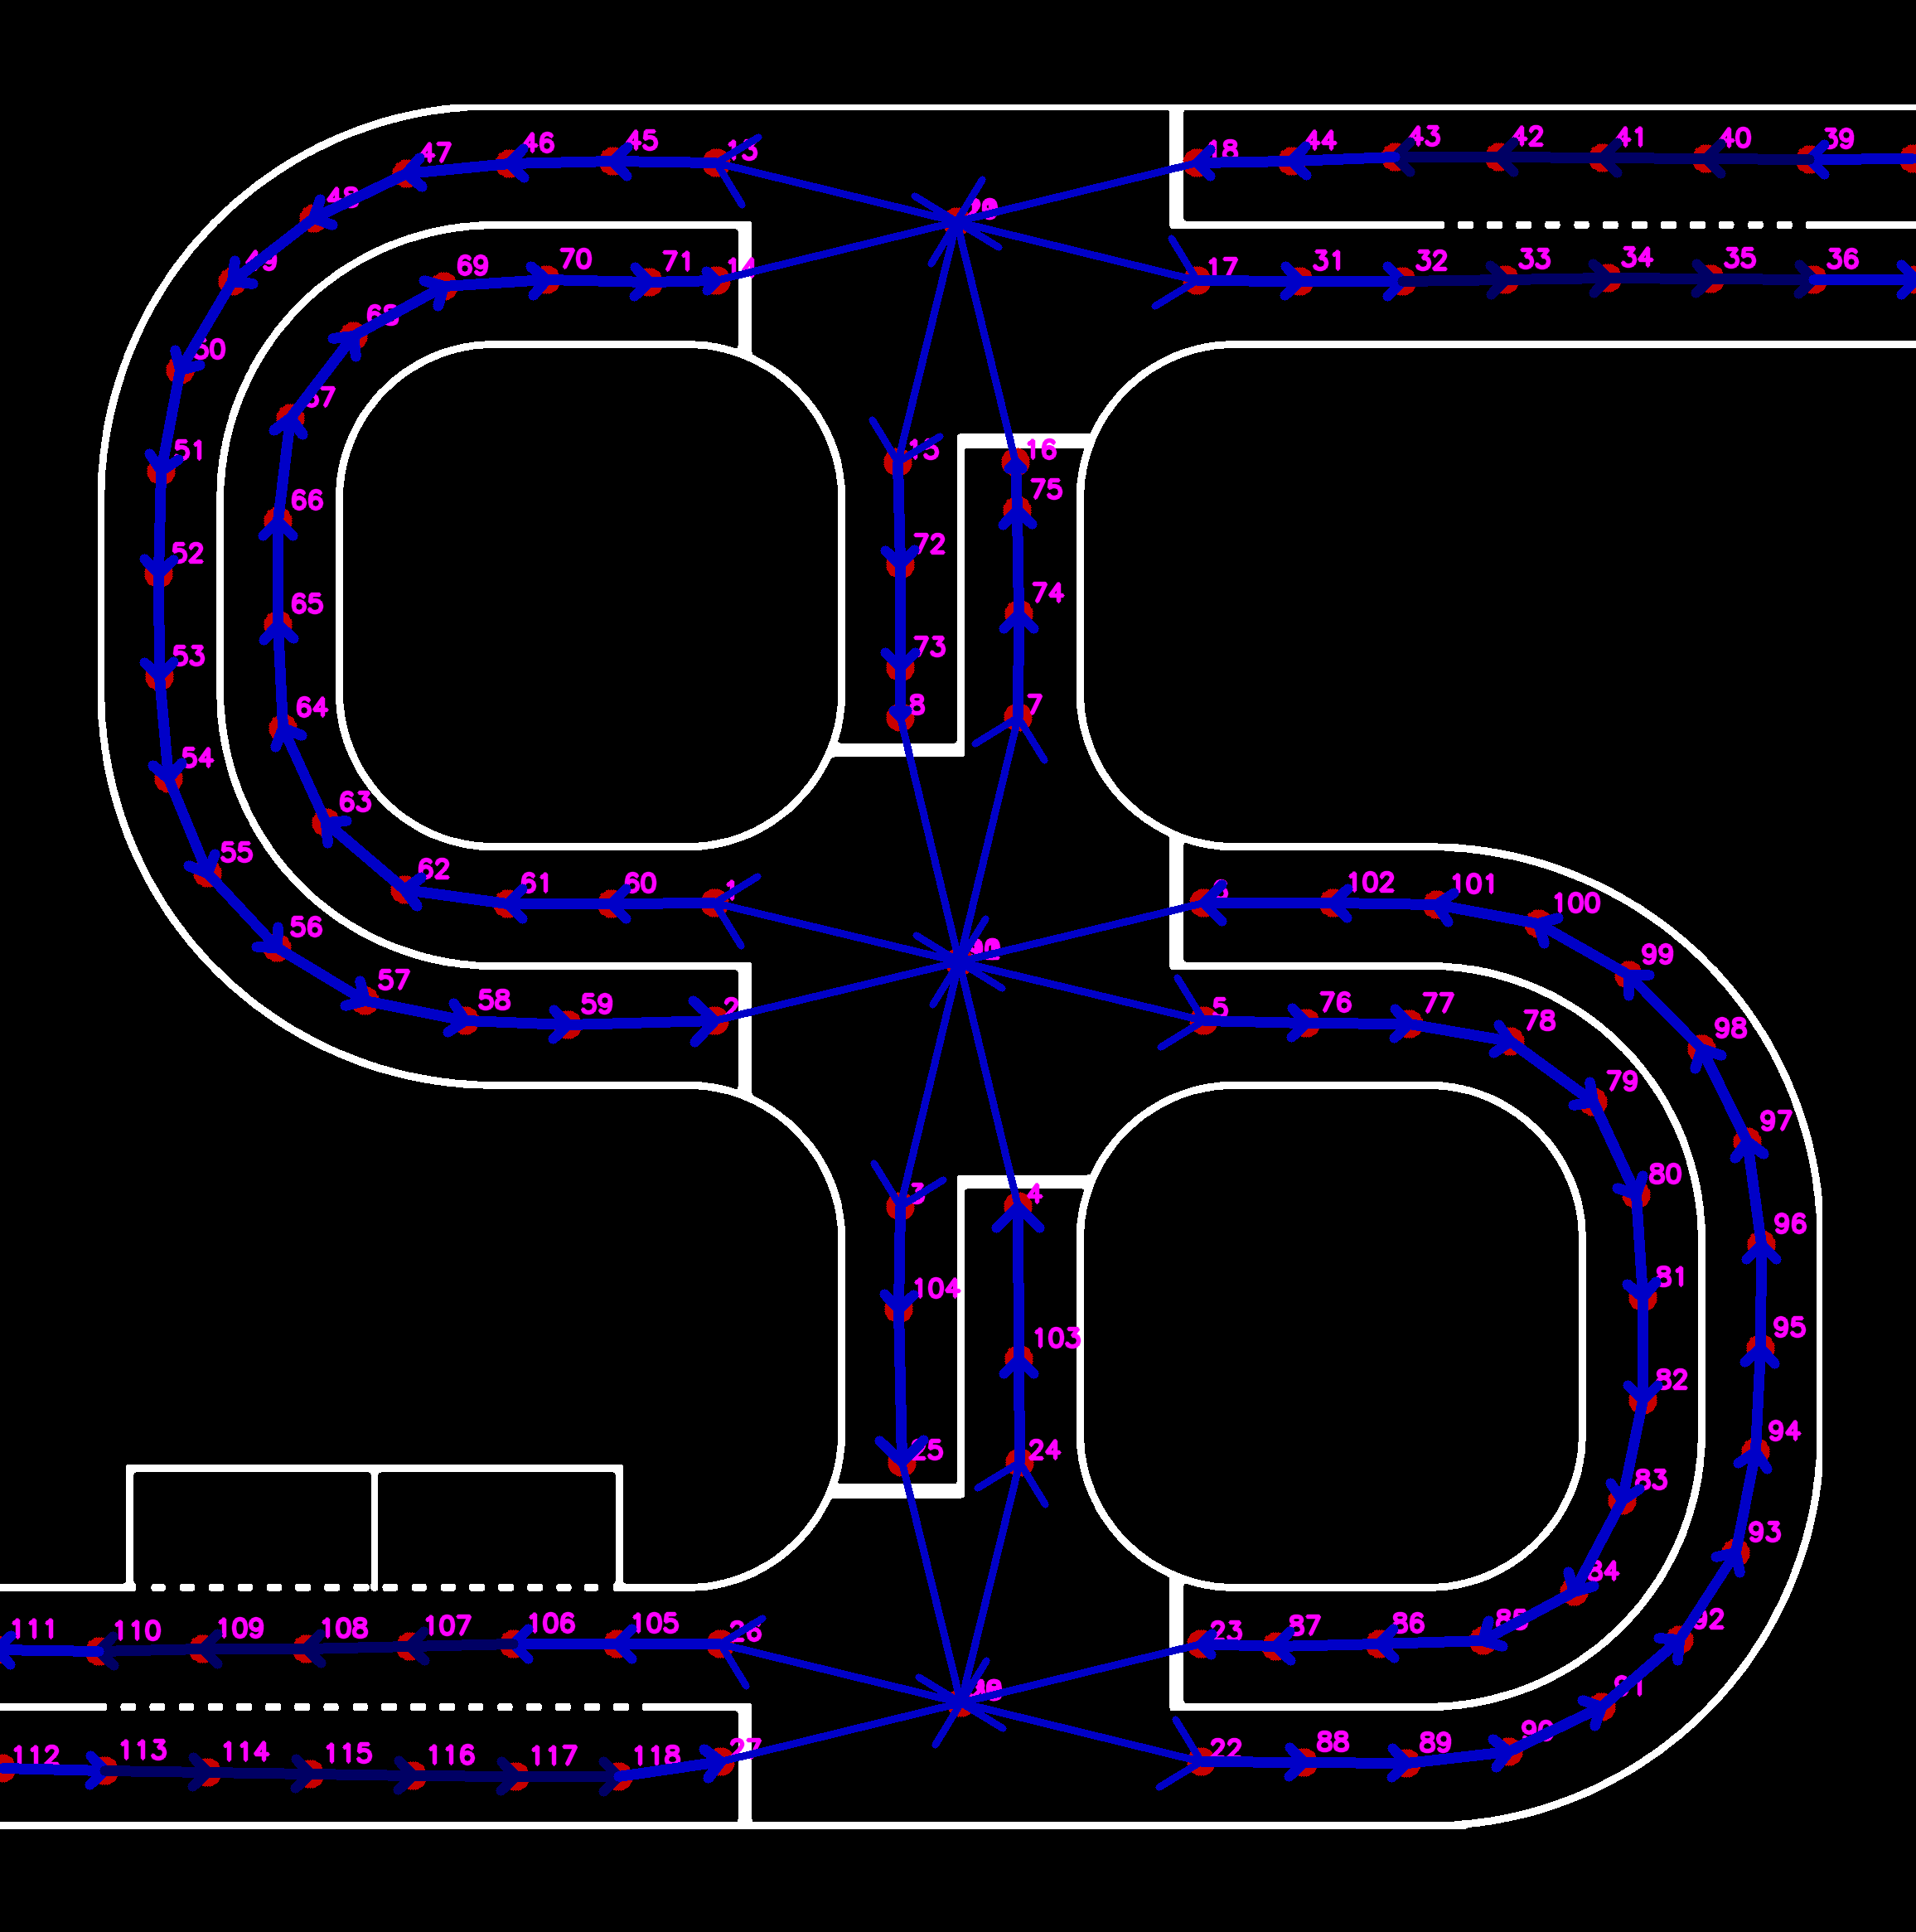
\includegraphics[height=10cm]{bilder/Test_track.png}
	\caption{Test-Track}
	\label{fig:testTrack}
\end{figure}

Der zweite Testfall testet den Algorithmus an einem weiteren einfachen Beispiel. Der Algorithmus soll im gegebenen Graphen den k�rzesten Weg zwischen den Knoten 57 und 17 finden. Dazu werden wie im vorherigen Testfall die Dateilesefunktion und der A*-Algorithmus aufgerufen und berechnete Pfad mit einem erwarteten Pfad verglichen. 

Der dritte Testfall �berpr�ft den A*-Algorithmus anhand eines komplexeren Beispiels. Dazu wird eine weitere GraphML-Datei eingelesen. Auch hier werden die Dateilesefunktion und der A*-Algorithmus aufgerufen und der berechnete Pfad mit einem vordefinierten Pfad verglichen. 
\newpage
Die Testf�lle dienen dazu, die Korrektheit und Effizienz der Implementierung des A*-Algorithmus zu �berpr�fen und sicherzustellen, dass er f�r verschiedene Szenarien korrekte Ergebnisse liefert. Wenn die tats�chlichen Pfade mit den erwarteten Pfaden �bereinstimmen, gelten die Tests als erfolgreich. Andernfalls wird eine Fehlermeldung ausgegeben und der Entwickler muss die Implementierung �berpr�fen, um m�gliche Fehler oder Optimierungsm�glichkeiten zu identifizieren. Die Testsuite stellt die robuste und zuverl�ssige Funktionalit�t des A*-Algorithmus in der Klasse sicher, was f�r die sichere Navigation im Graphennetzwerk in einer autonomen Fahrzeuganwendung von entscheidender Bedeutung ist.

\section{Leistungsvergleich des A*-Algorithmus: Ausf�hrungszeiten auf verschiedenen Graphen}
 In diesem Abschnitt werden Laufzeit und Speicherbedarf des A*-Algorithmus anhand von Benchmark-Tests verglichen. Die Tests wurden mit dem Google Benchmark Frame\-work durchgef�hrt, einer leistungsf�higen C++ Benchmark Suite, die von Google entwickelt wurde. Das Framework erm�glicht es Entwicklern, die Performance von C++-Code zu messen, verschiedene Implementierungen zu vergleichen und Engp�sse oder Performance-Probleme zu identifizieren. 
 
 Die Ergebnisse der Benchmark-Tests sind in der Tabelle \ref{tab:benchmark_erg} dargestellt, in der die Ausf�hrungszeit (Time), die CPU-Zeit (CPU) und die Anzahl der Iterationen (Iterations) f�r verschiedene Szenarien aufgelistet sind.

\begin{table}[h]
	\centering
	\begin{adjustbox}{width=\textwidth}
		\begin{tabular}{lrrr}
			\toprule
			Benchmark & Time & CPU & Iterations \\
			\midrule
			Simple & 4384524 ns & 2703059 ns & 237 \\
			Complex & 179371133 ns & 132812500 ns & 6 \\
			Multiple runs & 33912684 ns & 27832031 ns & 32 \\
			Multiple runs with competition track & 8878551100 ns & 6921875000 ns & 1 \\
			\bottomrule
		\end{tabular}
	\end{adjustbox}
	\caption{Benchmark-Ergebnisse des A*-Algorithmus}
	\label{tab:benchmark_erg}
\end{table}

Ein Blick auf die Tabelle zeigt einen deutlichen Unterschied in der Ausf�hrungszeit des A*-Algorithmus auf einfachen und komplexen Graphen. Die Ausf�hrungszeit auf einfachen Graphen betrug durchschnittlich etwa \SI{4}{\milli\second}, w�hrend auf komplexen Graphen durchschnittlich etwa \SI{179}{\milli\second} ben�tigt wurden. Diese Ergebnisse best�tigten die Erwartung, dass die Suche nach dem k�rzesten Weg auf einfachen Graphen weniger rechenintensiv ist.

Ein weiteres interessantes Ergebnis ist die Stabilit�t der Laufzeit bei wiederholter Ausf�hrung. Wie in Tabelle \ref{tab:benchmark_erg} zu sehen ist, zeigt der Benchmark-Test \glqq Multiple runs\grqq{} eine geringe Variation in den Laufzeiten. Dies deutet darauf hin, dass der Algorithmus konsistente und vorhersagbare Ergebnisse liefert, auch wenn es mehrmals ausgef�hrt wird. 
\newpage
Es ist wichtig anzumerken, dass sich die in dieser Analyse pr�sentierten Ergebnisse haupts�chlich auf die Ausf�hrungszeit beziehen. Die genaue Messung des Speicherbedarfs erfordert spezielle Werkzeuge und Mechanismen zur Ressourcen�berwachung, die in diesem Rahmen nicht durchgef�hrt wurden 

Die Ergebnisse der Benchmarks zeigen, dass der A*-Algorithmus einen leistungsf�higen Algorithmus zur Routenplanung darstellt. Die Laufzeit h�ngt jedoch stark von der Komplexit�t des zugrundeliegenden Graphen ab.


\newpage

\chapter{Fazit}

Die Implementierung des A*-Algorithmus in C++ erm�glichte ein tieferes Verst�ndnis der Funktionsweise des Algorithmus. Durch die praktische Umsetzung konnten die einzelnen Schritte des Algorithmus detailliert nachvollzogen und seine Funktionsweise verinnerlicht werden. Die Wahl der Heuristik und die effiziente Nutzung der Datenstrukturen erwiesen sich als entscheidend f�r die Leistungsf�higkeit des Algorithmus. Ein sorgf�ltige Auswahl der Heuristik kann die Effizienz des A*-Algorithmus erheblich verbessern und eine schnellere Suche nach dem optimalen Pfad erm�glichen. 

Die Evaluierung der Performance des A*-Algorithmus auf verschiedenen Graphen f�hrte zu interessanten Erkenntnissen. Es zeigte sich, dass die Laufzeit des Algorithmus stark von der Gr��e und Struktur des Graphen abh�ngt. In einfachen Graphen mit wenigen Knoten und Kanten konnte der A*-Algorithmus schnell eine optimale L�sung finden. In komplexeren Graphen mit vielen Knoten und Kanten stieg die Laufzeit jedoch deutlich an, da der Algorithmus eine umfangreichere Suche durchf�hren musste.

Allerdings wurden auch einige Grenzen des A*-Algorithmus aufgezeigt. In bestimmten Situationen, wie z.B. bei sehr komplexen Graphen ohne klar definierte Ziele, verlor der Algorithmus an Effizienz und n�herte sich dem optimalen Pfad nur langsam an. In solchen F�llen k�nnten alternative Routenplanungsalgorithmen, wie der Bellman-Ford-Algorithmus oder die Breitensuche bessere Ergebnisse liefern.

Abschlie�end ist festzuhalten, dass die Implementierung und Evaluierung des Routen\-planungsalgorithmus eine wertvolle Erfahrung war und ein fundiertes Verst�ndnis dieses leistungsf�higen Routen\-planungsalgorithmus erm�glicht hat. Die gewonnenen Erkenntnisse �ber die Leistungsf�higkeit und der Vergleich mit anderen Routenplanungsalgorithmen liefern wertvolle Informationen f�r zuk�nftige Anwendungen und Optimierungen des A*-Algorithmus.
\newpage


%\chapter{Zusammenfassung}
\blindtext[2]




% Alle Eintr�ge der BibTeX Datenbank "zitieren"
\nocite{*}
% Auswahl der BibTeX Datenbank f�r das Literaturverzeichnis
%\bibliography{literatur}
% Einstellen des Bibliography-Stils f�r das Literaturverzeichnis
%\bibliographystyle{plain}

\printbibliography


\noindent\begin{minipage}{\textwidth}
	% Abbildungsverzeichnis ausgeben
	\listoffigures
	% Tabellenverzeichnis ausgeben
	\listoftables
\end{minipage}
%\lstlistoflistings

% Anhang beginnen (Formatierung umschalten)
\appendix
\chapter{Anhang zum Systementwurf}
Allgemeine Beschreibung des Anhangs

\section{Diagramme}
Hier werden Diagramme platziert, die in den Textkapitel zuviel Platz beanspruchen.
\section{Tabellen}
Hier werden Tabellen platziert, die in den Textkapitel zuviel Platz beanspruchen.
\section{Quellcodelistings}
Hier werden Tabllen platziert, die in den Textkapitel zuviel Platz beanspruchen.


\end{document}
